%=====================================================================
%  main.tex  --  Overleaf-ready
%
%  Learning the Distribution Function: Normalizing-Flow Inference of
%  the Vertical Galactic Potential from Stellar Phase-Space Data
%
%  To compile on Overleaf: upload this file together with the `plots/`
%  directory (the figures referenced below live there).
%=====================================================================
\documentclass[11pt]{article}

\usepackage[utf8]{inputenc}
\usepackage[T1]{fontenc}
\usepackage{amsmath,amssymb}
\usepackage{graphicx}
\usepackage{booktabs}
\usepackage{siunitx}
\usepackage[margin=1in]{geometry}
\usepackage{caption}
\usepackage{subcaption}
\usepackage{xcolor}
\usepackage[colorlinks=true,linkcolor=blue,citecolor=blue,urlcolor=blue]{hyperref}

% figures are stored in the plots/ subdirectory
\graphicspath{{plots/}{./}}

% handy shorthands
\newcommand{\hdm}{h_{\mathrm{dm}}}
\newcommand{\zkms}{\,\mathrm{km\,s^{-1}}}
\newcommand{\pc}{\,\mathrm{pc}}
\newcommand{\Myr}{\,\mathrm{Myr}}
\newcommand{\ffo}{f_{0}}

\title{\bf Learning the Distribution Function:\\
Normalizing-Flow Inference of the Vertical Galactic Potential\\
from Stellar Phase-Space Data}

\author{Jonathan Kehat \and Oren Slone}

\date{\today}

%=====================================================================
\begin{document}
\maketitle

%---------------------------------------------------------------------
\begin{abstract}
The vertical structure of a stellar disk encodes the local gravitational
potential and hence the local dark-matter density. Inferring the potential
from a snapshot of stellar phase space is degenerate with the unknown
initial distribution function (DF) of the stars, $\ffo$: a wrong potential
can often be compensated by a suitably contrived $\ffo$. We study this
degeneracy in a controlled, one-dimensional setting. Stars are drawn from
an equilibrium DF in a realistic multi-component vertical potential,
optionally perturbed by a passing satellite, and evolved forward to produce
a mock ``observed'' phase-space distribution exhibiting the familiar
$z$--$w$ phase spiral. To recover the dark-matter scale height $\hdm$ we
back-integrate the observed stars under a trial potential and score the
resulting initial cloud against a model of $\ffo$; the potential is then
profiled by maximizing the likelihood over $\hdm$. The novelty is that
$\ffo$ is represented by a \emph{normalizing flow}, a flexible,
differentiable density model, rather than a fixed analytic form. We present
three tests of increasing difficulty --- a centered Gaussian $\ffo$, a
Gaussian with a bulk vertical streaming (shifted mean), and a genuinely
non-Gaussian (sharp-core, heavy-wing) velocity DF --- and we compare two
flow families: affine-coupling (RealNVP-type) flows and residual
(planar/Sylvester-type) flows. We find that the sharpness and location of
the recovered $\hdm$ depend not only on the flexibility of the flow but on
the match between the flow's low-capacity inductive bias and the true shape
of $\ffo$. The framework is deliberately data-agnostic: it applies to any
1D vertical phase-space sample and is not tied to a specific survey.
\end{abstract}

%=====================================================================
\section{Introduction}
\label{sec:intro}

The number density of stars in the vertical ($z$) direction near the
Galactic midplane, together with their vertical velocities ($w$), is a
classic probe of the local gravitational potential and of the local
dark-matter density $\rho_{\mathrm{DM}}$ (the ``Oort problem''). Modern
astrometric samples resolve the joint $(z,w)$ distribution in exquisite
detail, revealing that the disk is \emph{not} in perfect equilibrium: it
displays a coherent phase-space spiral, most naturally explained as the
ongoing phase mixing of a disturbance such as a satellite passage
\cite{widmark2021,antoja2018}.

Any attempt to read the potential off such a snapshot faces a fundamental
degeneracy: the observed distribution is the push-forward of an unknown
initial distribution function $\ffo$ through the (unknown) gravitational
dynamics. A biased potential can be partially absorbed by a distorted
$\ffo$. In this work we isolate and study this degeneracy in a clean,
one-dimensional simulation, and we ask a specific methodological question:
if $\ffo$ is modeled by an expressive, trainable density --- a normalizing
flow \cite{rezende2015,dinh2017,papamakarios2021} --- rather than a fixed
Gaussian, how well can the vertical potential (parameterized by the
dark-matter scale height $\hdm$) be recovered, and how does the answer
depend on the flow architecture?

The remainder of the paper is organized as follows.
Section~\ref{sec:sim} describes the phase-space simulation and the
inference pipeline. Section~\ref{sec:tests} presents the three density
tests. Section~\ref{sec:disc} discusses the results.
Appendix~\ref{app:flows} details the two normalizing-flow families used
throughout.

%=====================================================================
\section{The simulation and inference pipeline}
\label{sec:sim}

\subsection{Vertical potential and equilibrium DF}

We work in the one-dimensional, plane-parallel approximation of the
Widmark et al. vertical-disk model \cite{widmark2021}. The total vertical
potential is a sum of self-gravitating isothermal ($\mathrm{sech}^{2}$)
components representing the thin stellar disk, the thick disk and the gas,
plus a dark-matter component,
%
\begin{equation}
\Phi(z) \;=\; \sum_{i \in \{\mathrm{thin,thick,gas,DM}\}}
4\pi G\,\rho_{0,i}\, h_{i}^{2}\,
\ln\!\cosh\!\left(\frac{z}{h_{i}}\right),
\label{eq:phi}
\end{equation}
%
so that each component contributes a force
$\partial_z\Phi_i = 4\pi G\,\rho_{0,i}\,h_{i}\tanh(z/h_i)$. The dark-matter
term has midplane density $\rho_{\mathrm{DM}}$ and scale height $\hdm$;
throughout, the ground-truth value is $\hdm = 250\pc$. A key feature of
Eq.~\eqref{eq:phi} is that the midplane curvature $4\pi G\rho_{\mathrm{DM}}$
is \emph{independent} of $\hdm$: the scale height enters only through the
anharmonic ($\sim z^{4}/\hdm^{2}$ and higher) terms. Information on $\hdm$
therefore lives predominantly in the high-$|z|$, high-action stars, which
makes $\hdm$ intrinsically weakly constrained and is the physical origin of
the degeneracies studied here.

Each disk component is initialized in its \emph{equilibrium} DF,
$f_i(z,w) \propto \exp[-(\tfrac12 w^{2} + \Phi(z))/\sigma_{w,i}^{2}]$, i.e.\
an isothermal Gaussian in $w$ whose spatial profile is set self-consistently
by the full potential. The initial vertical-velocity distribution is thus
Gaussian by construction; the density tests of
Section~\ref{sec:tests} deliberately replace this with prescribed $\ffo$
shapes to probe the inference.

\subsection{Forward evolution and the phase spiral}

Stars are integrated with a leapfrog scheme under
Eq.~\eqref{eq:phi} for $t_{\mathrm{obs}} = 400\Myr$. A transient
perturbation --- a passing satellite modeled as a time-localized,
$\mathrm{sech}$-profile impulse $K_z(t,z)$ with a Gaussian envelope in time
--- can be switched on to seed a disequilibrium. Even without an explicit
satellite, an out-of-equilibrium initial cloud winds up into a spiral
through \emph{anharmonic phase mixing}: stars at different actions have
different vertical oscillation frequencies, so an initially smooth
overdensity shears into the characteristic $(z,w)$ spiral. This is
illustrated in Fig.~\ref{fig:before_after}: the equilibrium DF at $t=0$
(left), the evolved snapshot at $t=400\Myr$ (middle), and the
mean-subtracted relative overdensity $(n-\bar n)/\bar n$ (right), which
exposes the two-armed spiral residual that carries the disequilibrium
signal.

\begin{figure}[t]
  \centering
  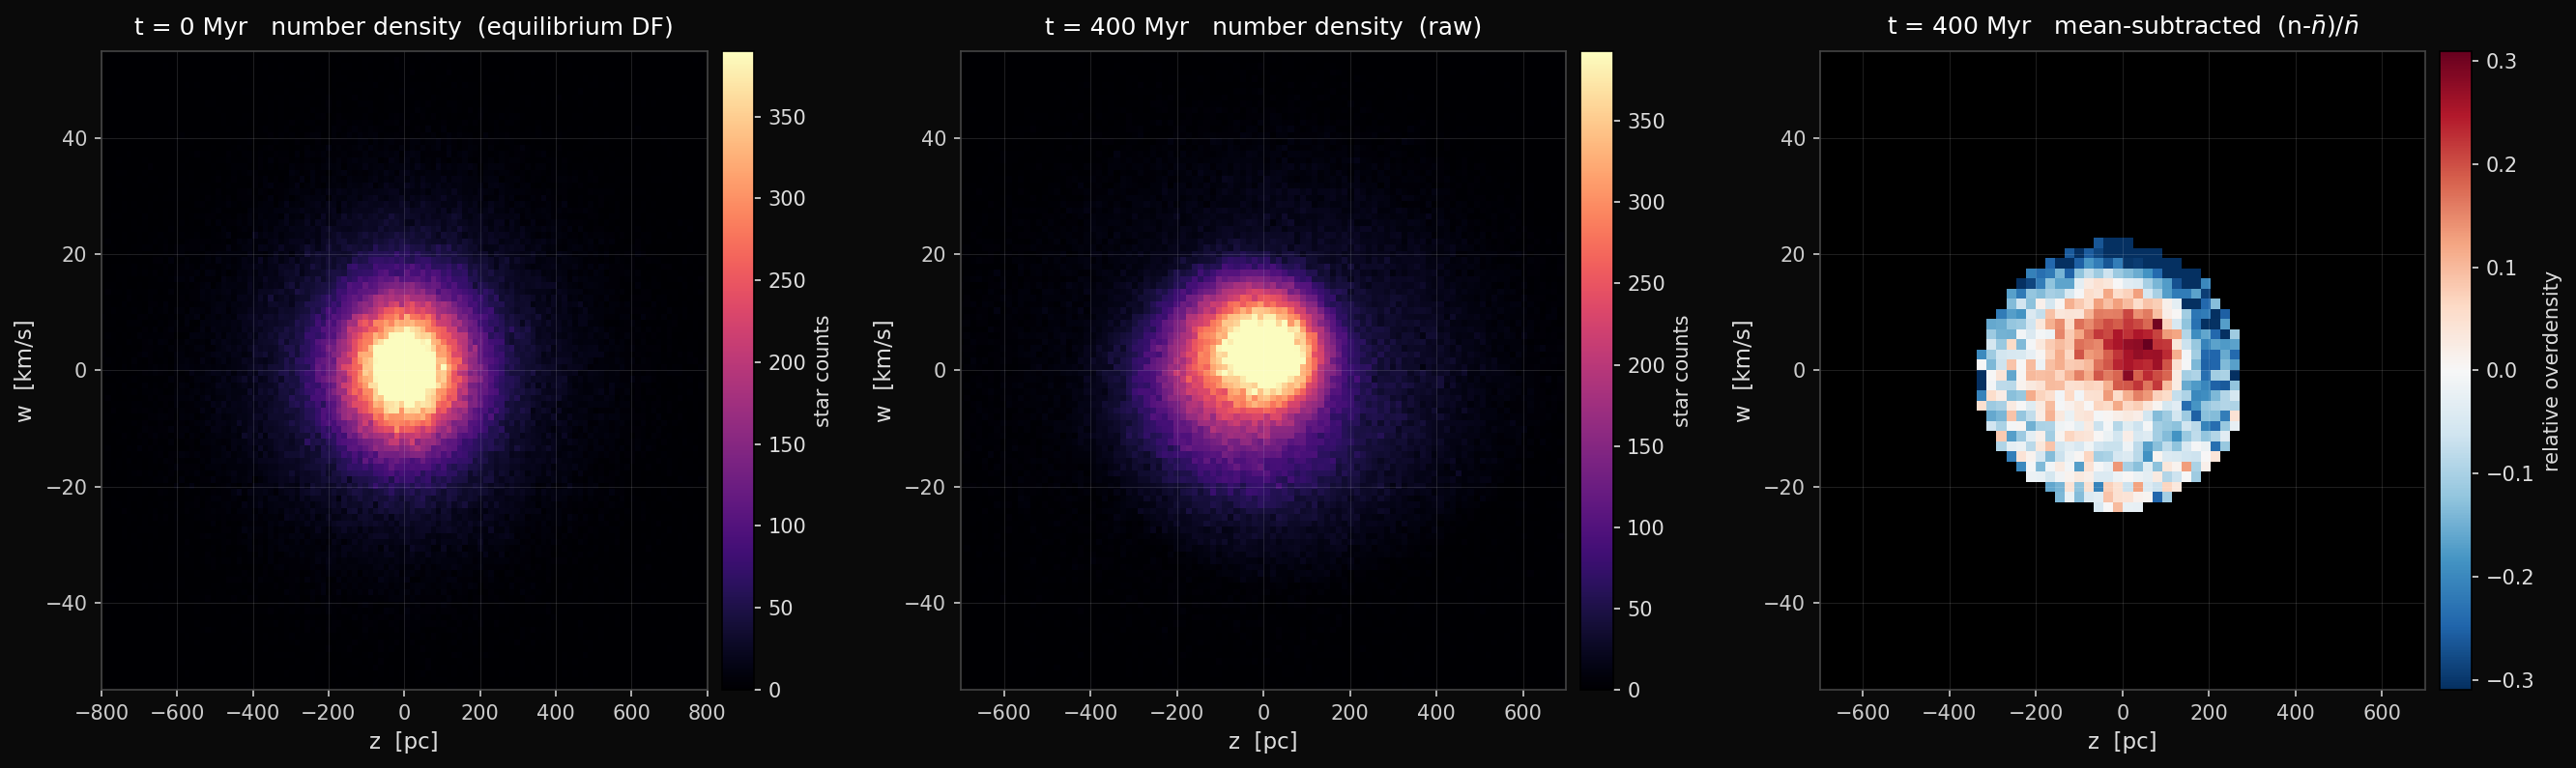
\includegraphics[width=\textwidth]{phase_space_before_after.png}
  \caption{Vertical phase space in the simulation. \textbf{Left:} the
  equilibrium distribution function at $t=0$. \textbf{Middle:} the raw
  number density at $t=400\Myr$ after forward evolution. \textbf{Right:}
  the mean-subtracted relative overdensity $(n-\bar n)/\bar n$, revealing
  the two-armed phase-space spiral produced by anharmonic phase mixing.}
  \label{fig:before_after}
\end{figure}

\begin{figure}[t]
  \centering
  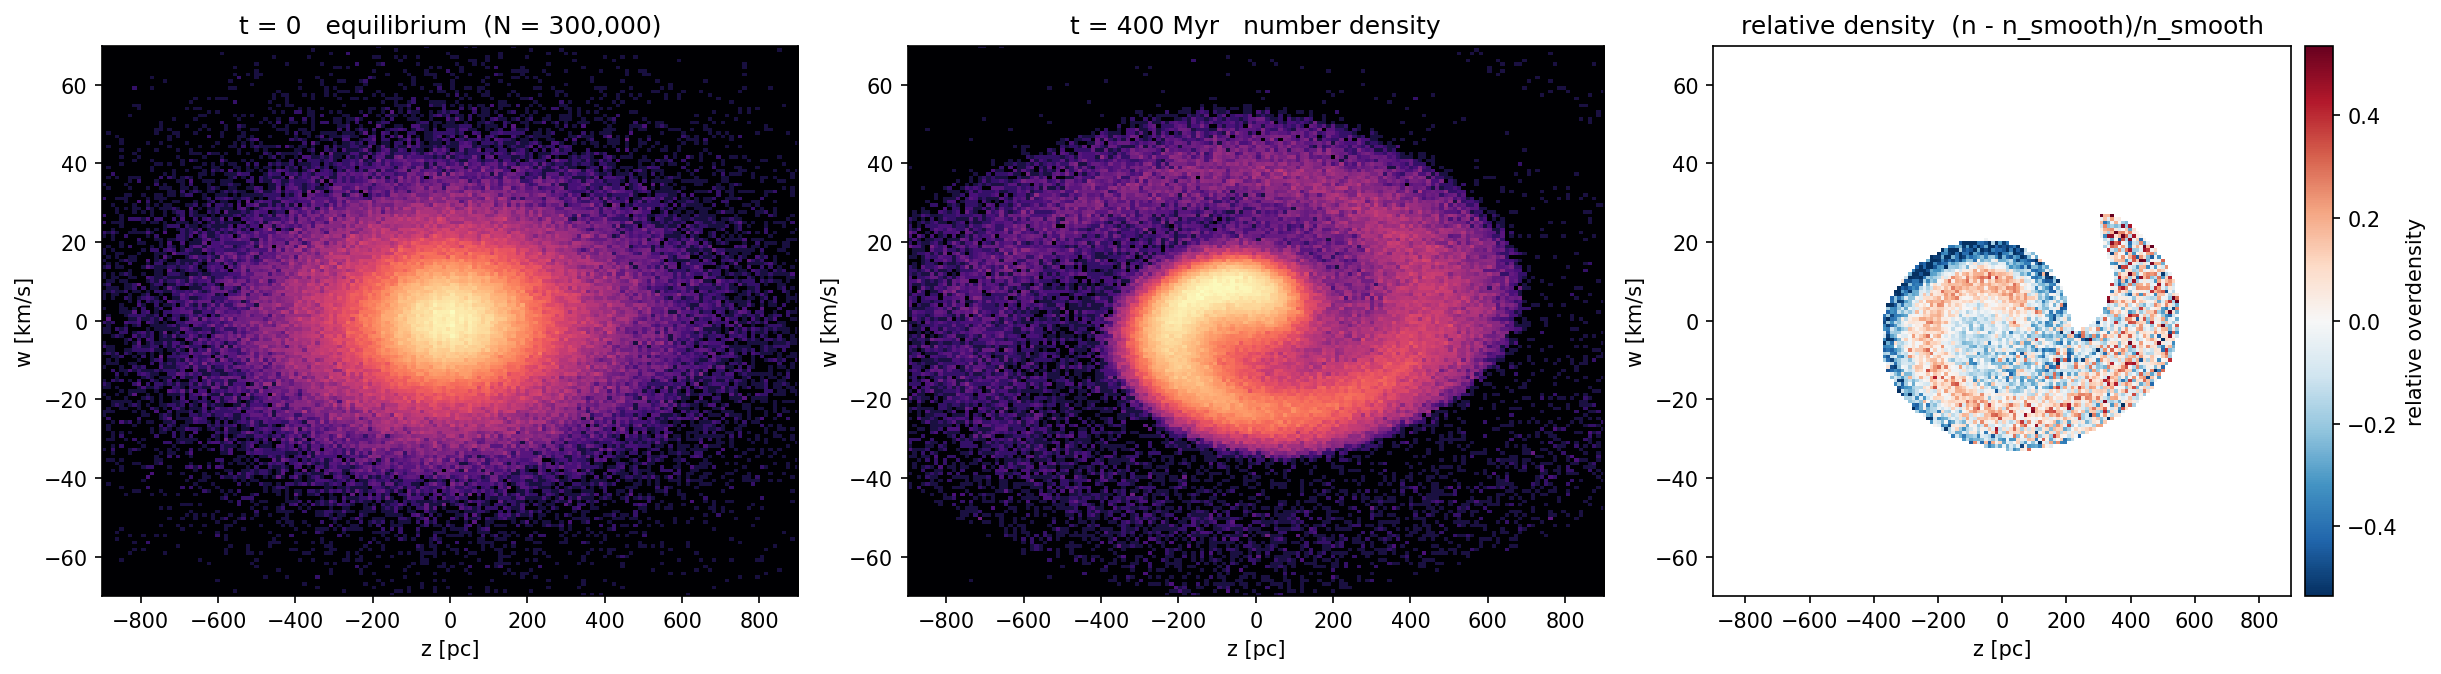
\includegraphics[width=0.72\textwidth]{spiral_widmark.png}
  \caption{Fully wound phase-space spiral produced by our pipeline
  (equilibrium DF plus a satellite perturbation), reproducing the
  qualitative morphology of the one-dimensional simulations of
  Widmark et al.\ \cite{widmark2021}. The spiral is an anharmonic phase-
  mixing feature; the satellite only seeds it.}
  \label{fig:spiral}
\end{figure}

\subsection{Inference by back-integration}
\label{sec:backint}

Given the ``observed'' snapshot $\{(z_j,w_j)\}$ at $t_{\mathrm{obs}}$, we
recover the potential as follows. For a trial dark-matter scale height
$\hdm$ we \emph{back-integrate} every star to $t=0$ under
Eq.~\eqref{eq:phi}, obtaining a candidate initial cloud
$\{(\hat z_j,\hat w_j)\}_{\hdm}$. By Liouville's theorem the DF is conserved
along orbits, so the correct $\hdm$ should map the observed distribution
back onto the true $\ffo$. We therefore score the back-integrated cloud
under a model density $q_\theta$ for $\ffo$ and minimize the negative
log-likelihood (NLL),
%
\begin{equation}
\mathrm{NLL}(\hdm,\theta) \;=\;
-\sum_j \ln q_\theta\!\big(\hat z_j,\hat w_j;\,\hdm\big),
\label{eq:nll}
\end{equation}
%
jointly over the potential parameter $\hdm$ and the density parameters
$\theta$. Profiling over $\theta$ at each $\hdm$ yields a profile likelihood
$\mathrm{NLL}(\hdm)$ whose minimum is the estimator $\hat h_{\mathrm{dm}}$
and whose curvature gives the (Wilks) uncertainty. When $q_\theta$ is a
fixed Gaussian this reduces to the standard vertical-Jeans-type analysis;
the contribution of this work is to let $q_\theta$ be a \emph{normalizing
flow}, a flexible differentiable density (Appendix~\ref{app:flows}), so
that the shape of $\ffo$ is learned rather than assumed.

%=====================================================================
\section{Density tests}
\label{sec:tests}

We now stress-test the pipeline with three prescribed initial DFs of the
separable form $\ffo(z,w) = \mathcal{N}(z;0,\sigma_z)\,g(w)$, differing only
in the velocity marginal $g(w)$. In each case we generate mock data with the
true $\ffo$, then profile $\mathrm{NLL}(\hdm)$ with the flow retrained to its
optimum at every $\hdm$. The ground truth is $\hdm = 250\pc$ in all three.

\subsection{Test 1 --- centered Gaussian $\ffo$}
\label{sec:test1}

The baseline test uses a centered Gaussian velocity DF,
$g(w)=\mathcal{N}(w;0,\sigma_w)$ --- the equilibrium case. This is the
easiest target: a low-capacity flow already represents it essentially
exactly, and the profile in Fig.~\ref{fig:prof_gauss} recovers a minimum
consistent with the truth. The profile is shallow (well depth of order a
few $\times10^{-3}$ nats), a direct reflection of the weak, purely
anharmonic dependence of the likelihood on $\hdm$ noted below
Eq.~\eqref{eq:phi}.

\begin{figure}[t]
  \centering
  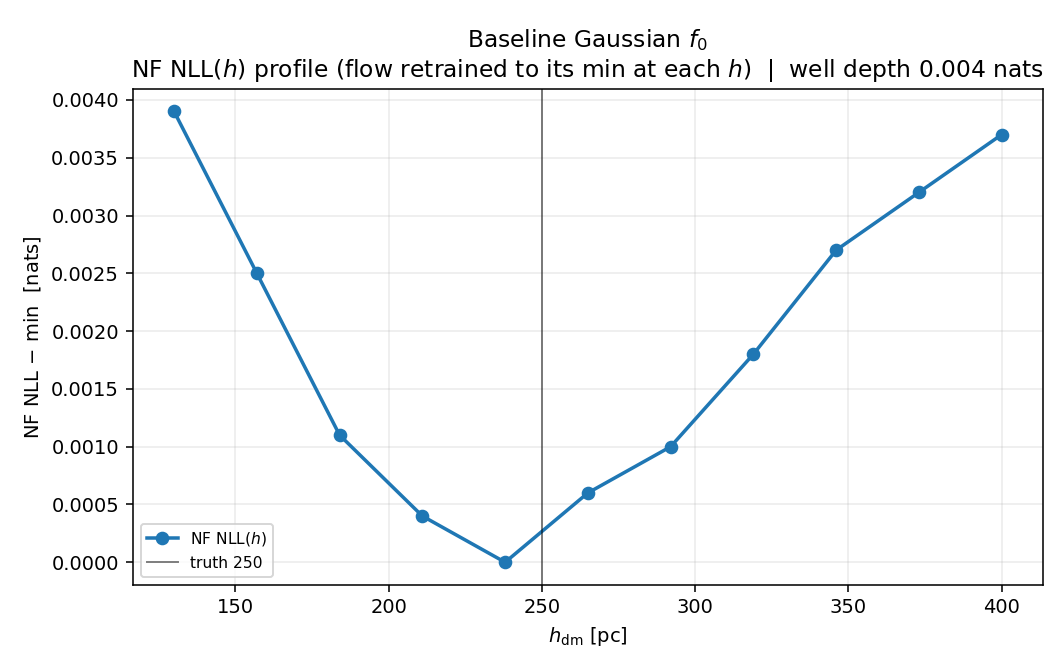
\includegraphics[width=0.70\textwidth]{nf_nll_profile_gaussian_f0.png}
  \caption{Test~1: profile likelihood $\mathrm{NLL}(\hdm)$ for a centered
  Gaussian $\ffo$, with the flow retrained to its minimum at each $\hdm$.
  The minimum sits at the true $\hdm = 250\pc$ (vertical line); the well is
  shallow because $\hdm$ enters the potential only anharmonically.}
  \label{fig:prof_gauss}
\end{figure}

\subsection{Test 2 --- shifted-mean Gaussian (bulk streaming)}
\label{sec:test2}

Here the velocity DF is a single Gaussian with a \emph{nonzero} mean,
$g(w)=\mathcal{N}(w;\,\mu_w,\sigma_w)$ with $\mu_w = 30\zkms$, representing a
net vertical streaming of the population at $t=0$. The shape is still
Gaussian, so an affine map captures it exactly, but the nonzero mean breaks
the $z\!\leftrightarrow\!w$ symmetry of the back-integrated cloud. The
profile (Fig.~\ref{fig:prof_shifted}) is again well-behaved, with a clean
minimum near the truth. Notably, in this test the \emph{residual} flow
locates the true $\hdm$ more robustly (across flow capacities) than the
affine-coupling flow: because a residual layer initializes near the identity
map, its low-capacity default is precisely ``a Gaussian, mildly deformed,''
which is the exact correct family for a shifted Gaussian. The coupling
flow's masked, one-coordinate-at-a-time factorization is a poorer match to
this simple target and yields a more scattered estimator
(cf.\ Appendix~\ref{app:flows}).

\begin{figure}[t]
  \centering
  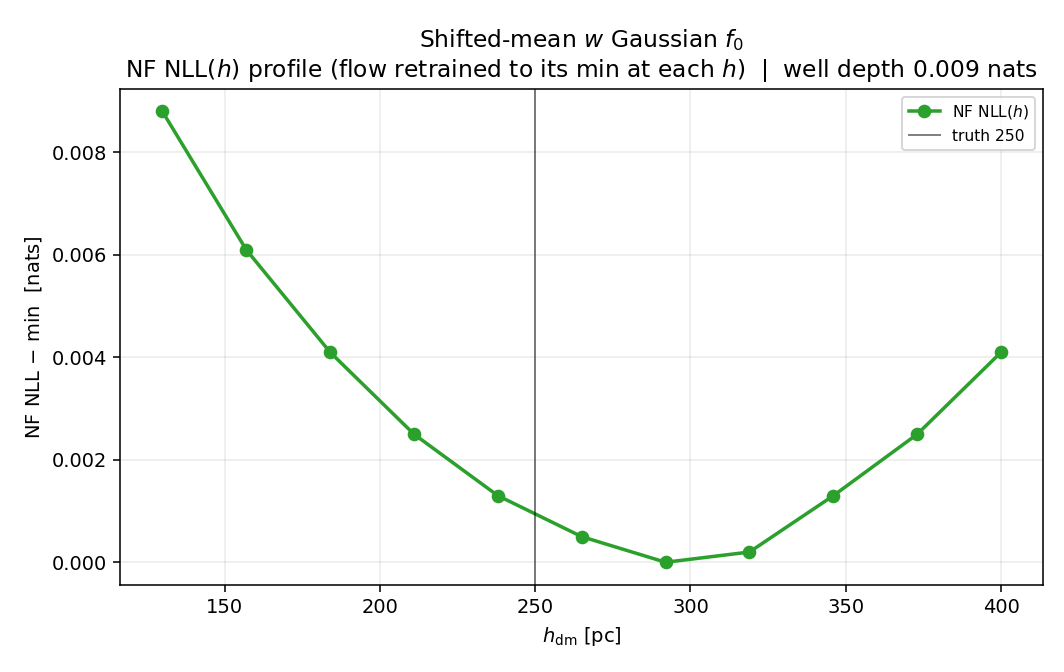
\includegraphics[width=0.70\textwidth]{nf_nll_profile_shifted_mean_w.png}
  \caption{Test~2: profile likelihood for a shifted-mean Gaussian $\ffo$
  ($\mu_w = 30\zkms$). The minimum brackets the true $\hdm = 250\pc$. The
  residual flow is more robust here than the coupling flow because a
  shifted Gaussian lies in the residual flow's near-identity default family
  (Appendix~\ref{app:flows}).}
  \label{fig:prof_shifted}
\end{figure}

\subsection{Test 3 --- non-Gaussian velocity DF (core + wings)}
\label{sec:test3}

The hardest test uses a genuinely non-Gaussian velocity DF: an
equal-mean mixture of a sharp core and heavy wings,
$g(w) = 0.6\,\mathcal{N}(w;0,\sigma_{\mathrm{core}})
      + 0.4\,\mathcal{N}(w;0,\sigma_{\mathrm{wing}})$
with a large width contrast --- a peaked, leptokurtic profile that no linear
map can reproduce. Now the flow's inductive bias is put to the test: a
low-capacity residual flow, whose default is Gaussian, \emph{under-fits} the
core+wings shape and biases $\hdm$, and only recovers the truth once
sufficient capacity is added; the coupling flow, built to warp shapes
nonlinearly, behaves differently again. The profile is shown in
Fig.~\ref{fig:prof_nongauss}. The lesson is that when $\ffo$ is non-Gaussian,
it is \emph{capacity}, not the choice of family, that controls the bias ---
in contrast to Test~2, where the near-Gaussian target rewarded the family
whose default already matched it.

\begin{figure}[t]
  \centering
  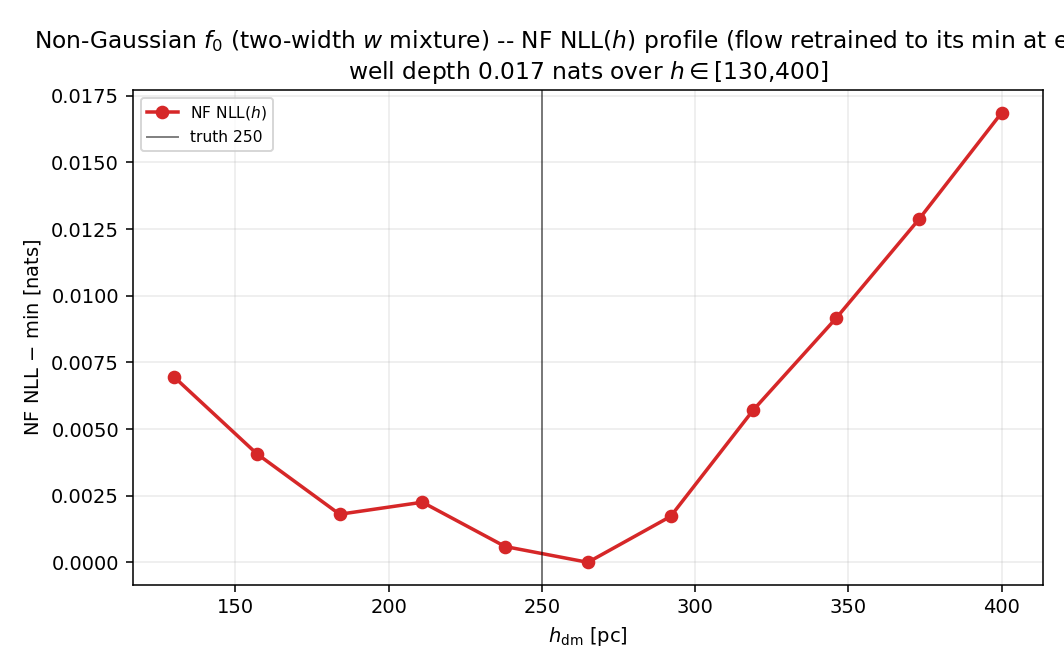
\includegraphics[width=0.70\textwidth]{nf_nll_profile_nongaussian_w_mixture.png}
  \caption{Test~3: profile likelihood for a non-Gaussian (sharp-core,
  heavy-wing) velocity DF. Recovering $\hdm$ now requires enough flow
  capacity to represent the leptokurtic shape; a near-identity default is
  no longer sufficient.}
  \label{fig:prof_nongauss}
\end{figure}

%=====================================================================
\section{Discussion}
\label{sec:disc}

Across the three tests a consistent picture emerges. The dependence of the
likelihood on $\hdm$ is intrinsically weak, because the scale height enters
the vertical potential only through anharmonic terms
(Eq.~\eqref{eq:phi}); the constraining power lives in the high-$|z|$ tail
of the distribution. When the modeled $\ffo$ matches the true shape, the
(shallow) profile minimum lands at the truth; when it does not, the flow can
partially absorb a biased potential into a distorted $\ffo$, displacing the
estimator. Which flow architecture performs best is therefore not a
question of raw flexibility --- with enough parameters both families are
comparably expressive --- but of whether the flow's \emph{low-capacity
default shape} matches the target: residual (planar/Sylvester) flows relax
toward a mildly deformed Gaussian and excel when $\ffo$ is near-Gaussian
(Test~2), whereas non-Gaussian targets (Test~3) simply demand more capacity
regardless of family. Because the entire pipeline operates on a generic
one-dimensional $(z,w)$ sample and an assumed potential family, it is
directly transferable to any vertical phase-space dataset.

%=====================================================================
\appendix

\section{The two normalizing-flow families}
\label{app:flows}

A normalizing flow models a density $q_\theta(\mathbf{y})$ as the
push-forward of a simple base density (here a standard 2D Gaussian
$p_Z$) through an invertible, differentiable map $T_\theta$ (a
\emph{bijection}, or ``transform''):
%
\begin{equation}
q_\theta(\mathbf{y}) \;=\;
p_Z\!\big(T_\theta(\mathbf{y})\big)\,
\left|\det \frac{\partial T_\theta}{\partial \mathbf{y}}\right|.
\label{eq:flow}
\end{equation}
%
Both families used in this work share the \emph{same} base distribution, the
\emph{same} input standardization, and the same likelihood assembly
(Eq.~\eqref{eq:flow}); they differ only in the bijection $T_\theta$ and in
the consequences that choice forces (the Jacobian structure and the
invertibility guarantee).

\paragraph{Affine-coupling (RealNVP-type) flows.}
A coupling layer \cite{dinh2015,dinh2017} splits the coordinates into two
blocks; one block is passed through unchanged and used to predict an affine
(scale-and-shift) transform of the other,
%
\begin{equation}
\mathbf{y}_A \mapsto \mathbf{y}_A, \qquad
\mathbf{y}_B \mapsto \mathbf{y}_B \odot \exp\!\big(s(\mathbf{y}_A)\big)
                 + t(\mathbf{y}_A).
\end{equation}
%
The Jacobian is triangular, so $\log|\det|$ is simply the sum of the scale
outputs, and the map is invertible \emph{by construction} for any weights.
Expressiveness is built up by stacking layers that alternate which block is
transformed. A single coupling layer, however, leaves one coordinate
untouched --- an intrinsic directional asymmetry that makes the smallest
coupling models rather rigid.

\paragraph{Residual (planar/Sylvester-type) flows.}
The second family uses a residual transform
%
\begin{equation}
\mathbf{y} \;\mapsto\; \mathbf{y} + V\,\tanh\!\big(W\mathbf{y} + b\big),
\label{eq:residual}
\end{equation}
%
with $W\in\mathbb{R}^{m\times d}$, $V\in\mathbb{R}^{d\times m}$. For $m=1$
this is exactly the \emph{planar flow} of Rezende \& Mohamed
\cite{rezende2015}; the multi-unit form in Eq.~\eqref{eq:residual} is the
\emph{Sylvester flow} generalization \cite{vandenberg2018}. (We refer to it
as ``residual'' by analogy with residual networks; note that the specific
construction termed \emph{Residual Flows} by Chen et al.\ \cite{chen2019}
--- invertible ResNets with spectral normalization and a stochastic
log-determinant estimator --- is a distinct object.) The map acts on both
coordinates jointly through a full $d\times d$ Jacobian
$\mathbf{I} + V\,\mathrm{diag}(1-\tanh^{2})\,W$, whose determinant is
computed explicitly. Unlike the coupling layer it is \emph{not} invertible
for arbitrary weights (it can fold if $\|VW\|$ is large), which is the price
of its symmetric treatment of the coordinates.

\paragraph{Why the choice matters.}
At equal parameter count the two families are comparably expressive, so the
differences seen in Section~\ref{sec:tests} are driven by their
\emph{low-capacity inductive bias}. The residual transform initializes near
the identity, so its default output is a Gaussian mildly perturbed --- the
exact right family for the near-Gaussian targets of Tests~1--2. The coupling
transform's default is a masked, one-coordinate-at-a-time affine warp, which
matches neither a plain shifted Gaussian nor a leptokurtic mixture
particularly well at low capacity. For strongly non-Gaussian $\ffo$
(Test~3), neither default suffices and additional capacity is required. A
general review of normalizing flows for density estimation and inference is
given in \cite{papamakarios2021}.

%=====================================================================
\begin{thebibliography}{9}

\bibitem{widmark2021}
A.~Widmark, C.~F.~P.~Laporte, and P.~F.~de~Salas,
\emph{Weighing the Galactic disk using phase-space spirals. I. Tests on
one-dimensional simulations},
Astron.\ Astrophys.\ \textbf{650}, A124 (2021).
\href{https://doi.org/10.1051/0004-6361/202140650}{doi:10.1051/0004-6361/202140650}.

\bibitem{antoja2018}
T.~Antoja et al.,
\emph{A dynamically young and perturbed Milky Way disk},
Nature \textbf{561}, 360 (2018).

\bibitem{rezende2015}
D.~J.~Rezende and S.~Mohamed,
\emph{Variational Inference with Normalizing Flows},
Proc.\ 32nd Int.\ Conf.\ on Machine Learning (ICML), PMLR \textbf{37}, 1530
(2015). \href{https://arxiv.org/abs/1505.05770}{arXiv:1505.05770}.

\bibitem{dinh2015}
L.~Dinh, D.~Krueger, and Y.~Bengio,
\emph{NICE: Non-linear Independent Components Estimation},
Workshop track, ICLR (2015). \href{https://arxiv.org/abs/1410.8516}{arXiv:1410.8516}.

\bibitem{dinh2017}
L.~Dinh, J.~Sohl-Dickstein, and S.~Bengio,
\emph{Density estimation using Real NVP},
Int.\ Conf.\ on Learning Representations (ICLR) (2017).
\href{https://arxiv.org/abs/1605.08803}{arXiv:1605.08803}.

\bibitem{vandenberg2018}
R.~van~den~Berg, L.~Hasenclever, J.~M.~Tomczak, and M.~Welling,
\emph{Sylvester Normalizing Flows for Variational Inference},
Proc.\ 34th Conf.\ on Uncertainty in Artificial Intelligence (UAI) (2018).
\href{https://arxiv.org/abs/1803.05649}{arXiv:1803.05649}.

\bibitem{chen2019}
R.~T.~Q.~Chen, J.~Behrmann, D.~Duvenaud, and J.-H.~Jacobsen,
\emph{Residual Flows for Invertible Generative Modeling},
Advances in Neural Information Processing Systems (NeurIPS) \textbf{32}
(2019). \href{https://arxiv.org/abs/1906.02735}{arXiv:1906.02735}.

\bibitem{papamakarios2021}
G.~Papamakarios, E.~Nalisnick, D.~J.~Rezende, S.~Mohamed, and
B.~Lakshminarayanan,
\emph{Normalizing Flows for Probabilistic Modeling and Inference},
J.\ Mach.\ Learn.\ Res.\ \textbf{22}(57), 1 (2021).
\href{https://arxiv.org/abs/1912.02762}{arXiv:1912.02762}.

\end{thebibliography}

\end{document}
